\documentclass[../main/main.tex]{subfiles}

\newdate{date}{11}{10}{2019}

\begin{document}

\section{Grancanonical potential}
\marginpar{ \textbf{Lecture 2.} \\  \displaydate{date}. \\ Compiled:  \today.}
The two intensive variables to became indipendent are \emph{T} and \( \mu  \). The corresponding Legendre transform is
\begin{equation}
  \Omega = U -T S - \sum_{i=1}^{r} \mu _i N _i = A - \sum_{i=1}^{r}  \mu _i N _ i
  \label{eq:}
\end{equation}
Differentiating this relation we obtain:
\begin{equation}
\begin{split}
\dd[]{\Omega }   &=  \dd[]{U} - S \dd[]{T} - T \dd[]{S} - \sum_{ij}^{} \dd[]{\mu _j} N_j - \sum_{i=1}^{r} \mu _i \dd[]{N_i}           \\
& = (\delta Q - T \dd[]{S}) - \delta W - S \dd[]{T} - \sum_{j=1}^{r} \dd[]{\mu _j} N_j - \sum_{j=1}^{r} \mu _j \dd[]{N_j}
\end{split}
  \label{eq:}
\end{equation}
Hence, \( \Omega = \Omega (T,P,{\mu _j}) \).
Internal energy $U$ and entropy $S$ are homogeneus function of the first order. A consequence of this fact is the relation called \textbf{Euler equation}:
\begin{equation}
  U = T S - P V + \sum_{j}^{} \mu _j N_j
  \label{eq:}
\end{equation}
Instead, the \textbf{Maxwell relations} are relations between the mixed derivatives of the thermodynamic potentials. They can be obtained from the expressions of \( \dd[]{U},\dd[]{H} ,\dd[]{A}, \dd[]{G}    \)  and \( \dd[]{\Omega }  \) and from the Schwarz theorem on mixed partial derivatives.
Due to Schwarz theorem, if a thermodynamic potential depends on \( t+1 \) variables there will be \( \frac{t(t+1)}{2} \)  indipendent mixed derivatives.
\begin{example}[Internal energy]
\begin{equation}
  \dd[]{U} = T \dd[]{S} - P \dd[]{V} + \mu \dd[]{N}
  \label{eq:2_1}
\end{equation}
where \( T = \qty(\pdv{U}{S} )_{V,N}  \) and  \( -P = \qty(\pdv{U}{V} )_{S,N}  \). It implies that
\begin{equation*}
        \pdv{U}{V}{S} = \qty(\pdv{T}{V} )_{S,N} \underset{\substack{ \text{from } \\  \text{Schwarz inequality} } }{=} -\qty(\pdv{P}{S} )_{V,N}
\end{equation*}
therefore, we have the \emph{1° Maxwell relation} :
\begin{equation*}
  \qty(\pdv{T}{V} )_{S,N} = -\qty(\pdv{P}{S} )_{V,N}
\end{equation*}
All the \emph{3 Maxweel relations} obtained by the differential \eqref{eq:2_1}
with \( t=2 \), for which we have \( t+1=3 \) and \( \frac{t(t+1)}{2}=3 \) (\( [S,V,N] \) ), are

\begin{subequations}
\begin{align}
  (S,V) &:& \qty(\pdv{T}{V} )_{S,N} =& - \qty(\pdv{P}{S} )_{V,N} & \\
  (S,N) &:& \qty(\pdv{T}{N} )_{V,S} =& \qty(\pdv{\mu }{S} )_{V,N} &\\
  (V,N) &:& -\qty(\pdv{P}{N} )_{S,V} =& \qty(\pdv{\mu }{V} )_{S,N} &
 \end{align}
\label{}
\end{subequations}
\end{example}

\begin{example}[Helmholz \( A=A(T,V,N) \)]
\begin{equation}
  \dd[]{A} = - S \dd[]{T} - P \dd[]{V} + \mu \dd[]{N}
\end{equation}
In this case the \emph{3 Maxweel relations} (\( [T,V,N] \) ) are
\begin{subequations}
\begin{align}
  (T,V) &:& \qty(\pdv{S}{V} )_{T,N} =&  \qty(\pdv{P}{T} )_{V,N} & \\
  (T,N) &:& -\qty(\pdv{S}{N} )_{T,V} =& \qty(\pdv{\mu }{T} )_{V,N} &\\
  (V,N) &:& -\qty(\pdv{P}{N} )_{V,T} =& \qty(\pdv{\mu }{V} )_{T,N} &
 \end{align}
\label{}
\end{subequations}
\end{example}
\begin{example}[Gibbs \( G=G(T,P,N) \) ]
  \begin{equation}
    \dd[]{G} = - S \dd[]{T} - V \dd[]{P} + \mu \dd[]{N}
  \end{equation}
  In this case the \emph{3 Maxweel relations} (\( [T,P,N] \) ) are
  \begin{subequations}
  \begin{align}
    (T,P) &:& -\qty(\pdv{S}{P} )_{T,N} =&  \qty(\pdv{V}{T} )_{P,N} & \\
    (T,N) &:& -\qty(\pdv{S}{N} )_{T,P} =& \qty(\pdv{\mu }{T} )_{P,N} &\\
    (P,N) &:& \qty(\pdv{V}{N} )_{P,T} =& \qty(\pdv{\mu }{P} )_{T,N} &
   \end{align}
  \label{}
  \end{subequations}
\end{example}

\section{Response functions}
Aim of most experiments is to measure the response of a thermodynamic system write respect to controlled variatious of thermodynamic variables. In fact, any osservation is just the pertubation of a system and looking for the response.
A list of the commonly used response functions is the following:
\begin{itemize}
\item \emph{Thermal expansion coefficient at constant pressure}.
\begin{equation}
  \alpha _P \equiv \frac{1}{V} \qty(\pdv{V}{T} )_{P,N}
  \label{eq:}
\end{equation}
\item \emph{Molar heat capacity at constant pressure}.
\begin{equation}
  c_P = \qty(\frac{\delta Q}{\dd[]{T} } )_P = T \qty(\pdv{S}{T} )_P \underset{-S=\qty(\pdv{G}{T} )_P }{=}  - T \qty(\pdv[2]{G}{T} )_P
  \label{eq:}
\end{equation}
\item \emph{Adiabatic compressibility}.
\begin{equation}
  k_S = -\frac{1}{V} \qty(\pdv{V}{P} )_{S,N} \underset{V=\qty(\pdv{H}{P} )_{S,N} }{=} - \frac{1}{V} \qty(\pdv[2]{H}{P} )_{S,N}
    \label{eq:}
\end{equation}
\item \emph{Isothermal compressibility} .
\begin{equation}
  k_T = -\frac{1}{V} \qty(\pdv{V}{P} )_{T,N} \underset{V=\qty(\pdv{G}{P} )_{T,N} }{=} - \frac{1}{V} \qty(\pdv[2]{G}{P} )_{T,N}
  \label{eq:}
\end{equation}
\begin{remark}
Remember that \( k_T \) it is the second derivative of the Gibbs potential write respect to pressure.
\end{remark}
\item \emph{Specific heat at constant volume}. Consider a quasi static transformation.
\begin{equation}
  c_V =  \qty(\frac{\delta Q}{\dd[]{T} } )_{V,N} = T \qty(\pdv{S}{T} )_{V,N}
      = \qty( \frac{\partial{(-\partial{A}/\partial{T} )_{V,N}} }{\partial{T} })_{V,N}
      = - T \qty(\pdv[2]{A}{T} )_{V,N}
  \label{eq:}
\end{equation}
\item \emph{Magnetic suscettibility (d=1)} for a magnetic system \( (\va{M},\va{H},T  ) \).
\begin{equation}
  \chi_T = \qty(\pdv{M}{H} )_T \underset{M = -\eval{\pdv{G}{H}}_T }{=}  - \qty(\pdv[2]{G}{H} )_T
  \label{eq:}
\end{equation}
More generals, \( \va{M},\va{H}   \) we have
\begin{equation}
  \chi _{\alpha \beta } = \qty(\pdv{M_ \alpha }{H_ \beta } )_T , M_ \alpha = -\eval{\pdv{G}{H_ \alpha }}_T \Rightarrow \chi _{\alpha \beta } = \eval{\pdv{G}{H_ \beta }{H_ \alpha }}_T
  \label{eq:}
\end{equation}

\end{itemize}
Note that the response functions, when used with the Maxwell relations, allow to express observables usually inaccessible to experiments with measurable quantitities.
\begin{example}[The Maxwell relation]
  \begin{equation*}
    \qty(\pdv{S}{P} )_{T,N} = - \qty(\pdv{V}{T} )_{P,N}
  \end{equation*}
  obtained from
  \begin{equation*}
\dd[]{G} = - S \dd[]{T} + V \dd[]{P}
  \end{equation*}
and the response function \( \alpha _P \) permit to write
\begin{equation}
  \underbrace{\qty(\pdv{S}{P} )_{T,N}}_{\substack{ \text{inaccessible} \\  \text{to experiments} } }  = \underbrace{- V \alpha _P}_{\text{measurable}}
  \label{eq:}
\end{equation}
\end{example}
\begin{example}
Let us start with the Maxwell relation
\begin{equation*}
  \qty(\pdv{S}{V} )_{T,N} =  \qty(\pdv{P}{T} )_{V,N}
\end{equation*}
obtained from
\begin{equation*}
    \dd[]{A} = - S \dd[]{T} - P \dd[]{V} + \mu \dd[]{N}
\end{equation*}
From some property of multi-variable differential calculus one has the \textbf{triple product rule}:
\begin{equation}
    \qty(\pdv{P}{T} )_{V,N}  \qty(\pdv{V}{P} )_{T,N}   \qty(\pdv{T}{V} )_{P,N} =-1
  \label{eq:}
\end{equation}
Hence
\begin{equation}
\begin{split}
    \qty(\pdv{P}{T} )_{V,N} &= \frac{-1}{ \qty(\pdv{V}{P} )_{T,N}   \qty(\pdv{T}{V} )_{P,N} }  = - \frac{  \qty(\pdv{V}{T} )_{P,N} }{   \qty(\pdv{V}{P} )_{T,N} } \\
    &= \frac{-V \alpha _P}{-V k_T} = \frac{\alpha _P}{k _T}
\end{split}
  \label{eq:}
\end{equation}
\end{example}

\section{Response functions and thermodynamic stability}
Now, we analyze the concept of \textbf{thermal stability}. If one injects heat in a system either at constant volume or at constant pressure, its temperature will inevitably increase
\begin{equation}
  \begin{cases}
   c_V \equiv \qty(\frac{\delta Q}{\dd[]{T} })_V \ge 0  \\
   c_P \equiv \qty(\frac{\delta Q}{\dd[]{T} })_P \ge 0
  \end{cases}
\label{eq:}
\end{equation}
\begin{remark}
The thermal capacities are \emph{non-negative functions}!
\end{remark}
It is useful also the concept of \textbf{mechanical stability}. If one compress a system by keeping \emph{T} constant, we would expect that it shrinks
\begin{equation}
  k_T = - \frac{1}{V} \qty(\pdv{V}{P} )_T \ge 0
  \label{eq:}
\end{equation}
Similar considerations for a magnetic system, gives
\begin{equation}
  c_H \ge 0, \quad c_M \ge 0, \quad \chi_M \ge 0
  \label{eq:}
\end{equation}
\begin{remark}
In diamangetic systems \( \chi_M \) can also be negative.
\end{remark}

\begin{exercise}
By using Maxwell relations show that
\begin{subequations}
\begin{align}
  c_P - c_V &= \frac{T V \alpha ^2}{k_T} = \frac{1}{V k_T} T \qty(\pdv{V}{T} )_P^2 \\
  c_H - c_M &= \frac{T}{\chi _T} \qty(\pdv{M}{T} )_H^2
\end{align}
\label{}
\end{subequations}
\end{exercise}
\noindent A consequence is that since the right hand terms are non negative it follows that
\begin{equation}
  \begin{cases}
   c_P \ge c_V \ge 0  \\
   c_H \ge c_M \ge 0
  \end{cases}
\label{eq:}
\end{equation}

For reasuming, we have seen the thermodynamic of a phase, where the equilibrium state can be described by the maximum of the entropy. If we have a given phase, we can look for the Gibbs function. If we have more phases, we want to change between these phases.

\section{}

Consider a fluid system and the variable \( \frac{G}{N} \equiv g = g (T,P) \), where \( g \) is not anymore a function of \emph{N}  because we have divided for \emph{N} . Suppose that \( \alpha  \) is in a given phase that can be \emph{liquid}, \emph{gas}, \emph{solid}. Therefore \( g_ \alpha  \)  is a function of \emph{T,P}, where new value of \emph{T}  and \emph{P}  corresponds to the minimum of \( g_ \alpha \). Consider the surface \( g_ \alpha  \) and
\( g_ \beta  \), we are looking for the lower one (see Figure \ref{fig:2_1}) and there is a moment in which they coexist and the projection of the intersection is called projection line for which \( g_ \alpha(T,P) = g_ \beta(T,P) \).


\begin{figure}[h!]
\centering
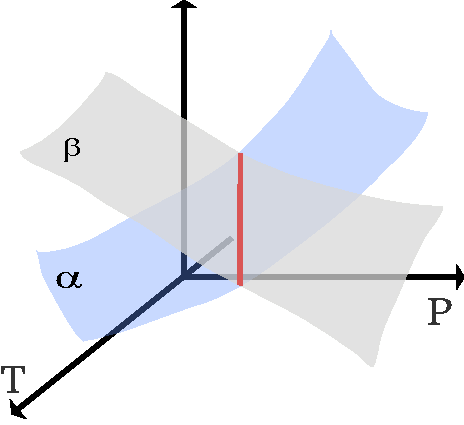
\includegraphics[width=0.4\textwidth]{../lessons/2_image/1.pdf}
\caption{\label{fig:2_1} Description.}
\end{figure}

\noindent Now, we fix \( P = P^* \), we have \( g_ \alpha (T,P^*) \) as shown in Figure \ref{fig:2_2}. Remember \( c_P = - T \qty(\pdv[2]{G}{T}) \ge 0 \) , it is a concave function.
At the triple point \( g_{\text{solid}}(T_ \alpha, P^*) = g_{\text{liq}}(T_a) \) and \( g_{\text{liq}}(T_b) = g_{\text{gas}}(T_b , P^*) \) (see Figure \ref{fig:2_3} ).

\begin{figure}[h!]
\begin{minipage}[c]{0.5\linewidth}
\subfloat[][Description]{ 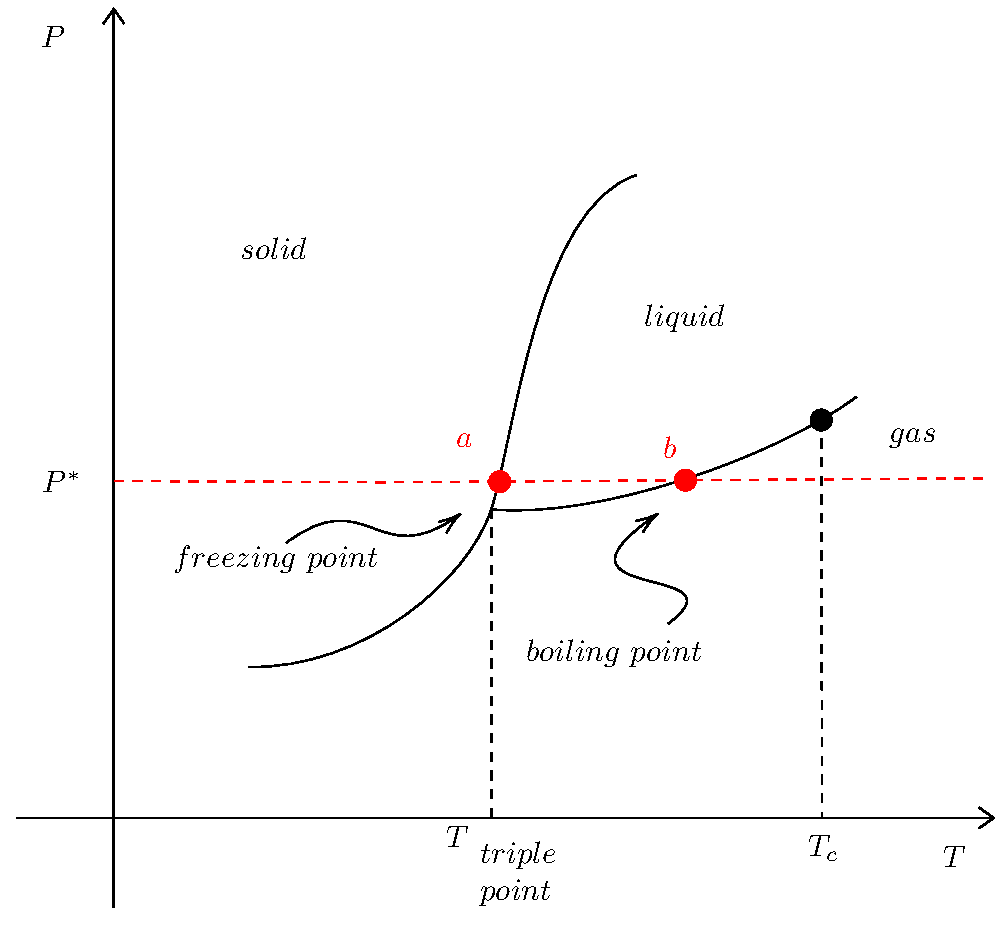
\includegraphics[width=0.8\textwidth]{../lessons/2_image/2.pdf}  \label{fig:2_2} }
\end{minipage}
\begin{minipage}[]{0.5\linewidth}
\centering
\subfloat[][Description]{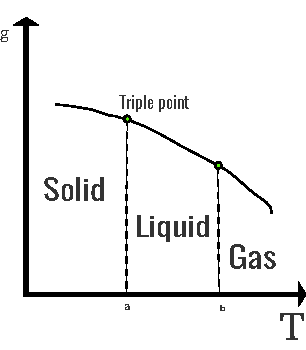
\includegraphics[width=0.8\textwidth]{../lessons/2_image/3.pdf}  \label{fig:2_3} }
\end{minipage}
\caption{\label{fig:} Description}
\end{figure}

If we define \( s=-\qty(\pdv{g}{T} )_P  \), we have \( \Delta s T \) that is called the \emph{latent heat} (Figure \ref{fig:2_4})
\begin{figure}[h!]
\centering
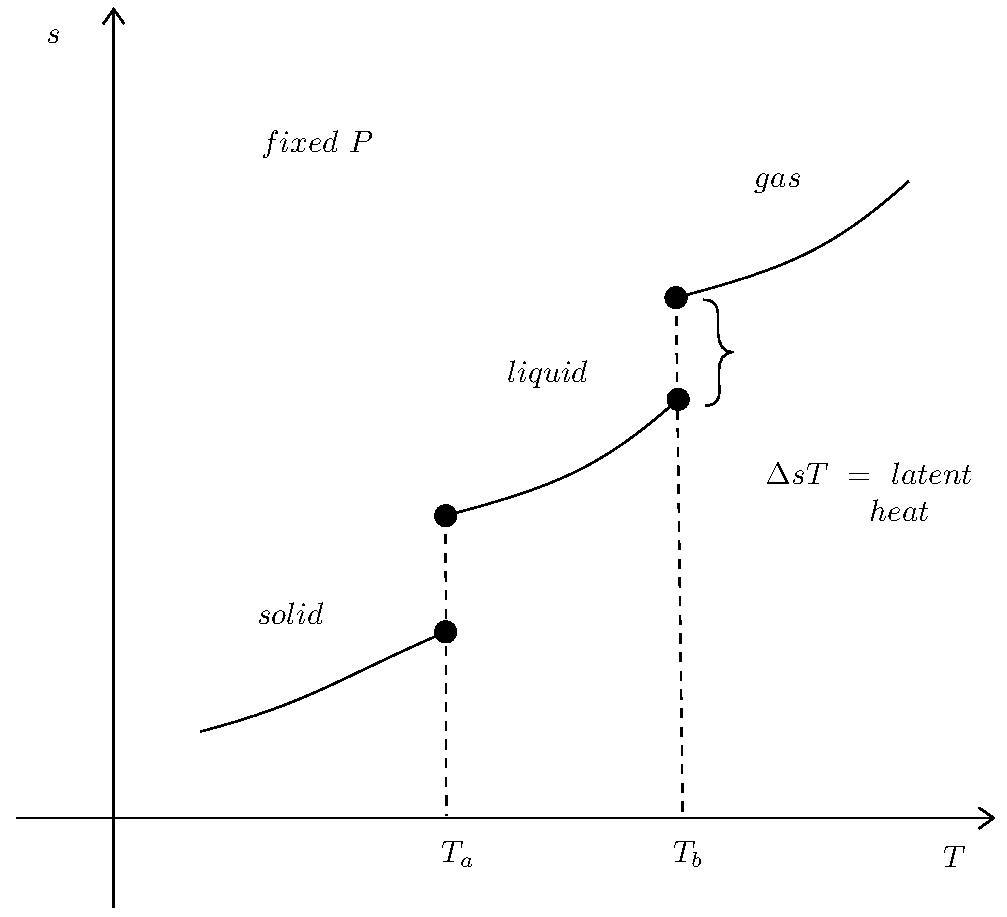
\includegraphics[width=0.4\textwidth]{../lessons/2_image/4.pdf}
\caption{\label{fig:2_4} Description.}
\end{figure}

There are other cases in which we do not have this effect, as in Figure \ref{fig:2_5}. This is different from the previous situation in which we had a jump.
\begin{figure}[h!]
\begin{minipage}[c]{0.3\linewidth}
\subfloat[][Description]{ 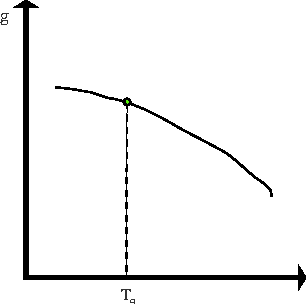
\includegraphics[width=0.8\textwidth]{../lessons/2_image/5.pdf}  \label{fig:} }
\end{minipage}
\begin{minipage}[]{0.3\linewidth}
\centering
\subfloat[][Description]{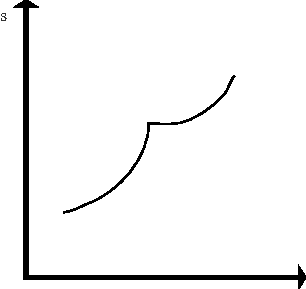
\includegraphics[width=0.8\textwidth]{../lessons/2_image/6.pdf}  \label{fig:} }
\end{minipage}
\begin{minipage}[]{0.3\linewidth}
\centering
\subfloat[][Description]{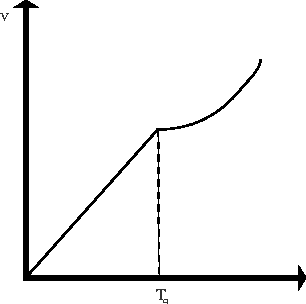
\includegraphics[width=0.8\textwidth]{../lessons/2_image/7.pdf}  \label{fig:} }
\end{minipage}
\caption{\label{fig:2_5} Description}
\end{figure}

If we look for example at the specific heat in Figure \ref{fig:2_6}, it represent the transition from superconduction.
\begin{figure}[h!]
\centering
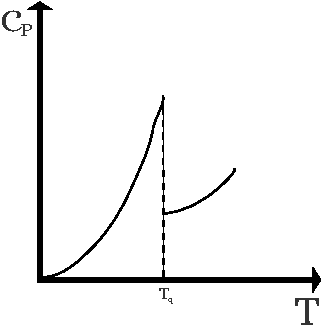
\includegraphics[width=0.5\textwidth]{../lessons/2_image/8.pdf}
\caption{\label{fig:2_6} Description.}
\end{figure}

The critical point is special beacause there is not a jump, so we can go continuously from gas to liquid. The response function when we plot this point shows that the specific heat diverges.
The transitions are classified in the first order transition and continuous transition. The superfluid transition is a transition where the second derivative of the thermodynamic potential diverges. There are many phase transitions that can be classified in different ways.
We note that at the coexistence line we increase V, but the pression remains constant. At the coexistence line we see bubbles. It is the density that is changing locally, the bubbles becames bigger and bigger and at the \( V_G \) , becames a liquid.
Usually critical points are end point of first order transition phases. Why there is no critical point between solid and liquid? Landau point. There is a break of symmetry, for instance we can think about the structure of the bravais lattice. Instead, from gas to liquid symmetries are not broken.

\begin{figure}[h!]
\begin{minipage}[c]{0.5\linewidth}
\subfloat[][Description]{ 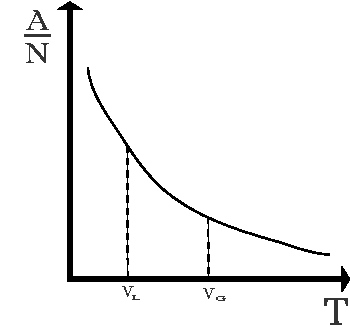
\includegraphics[width=0.8\textwidth]{../lessons/2_image/9.pdf}  \label{fig:} }
\end{minipage}
\begin{minipage}[]{0.5\linewidth}
\centering
\subfloat[][Description]{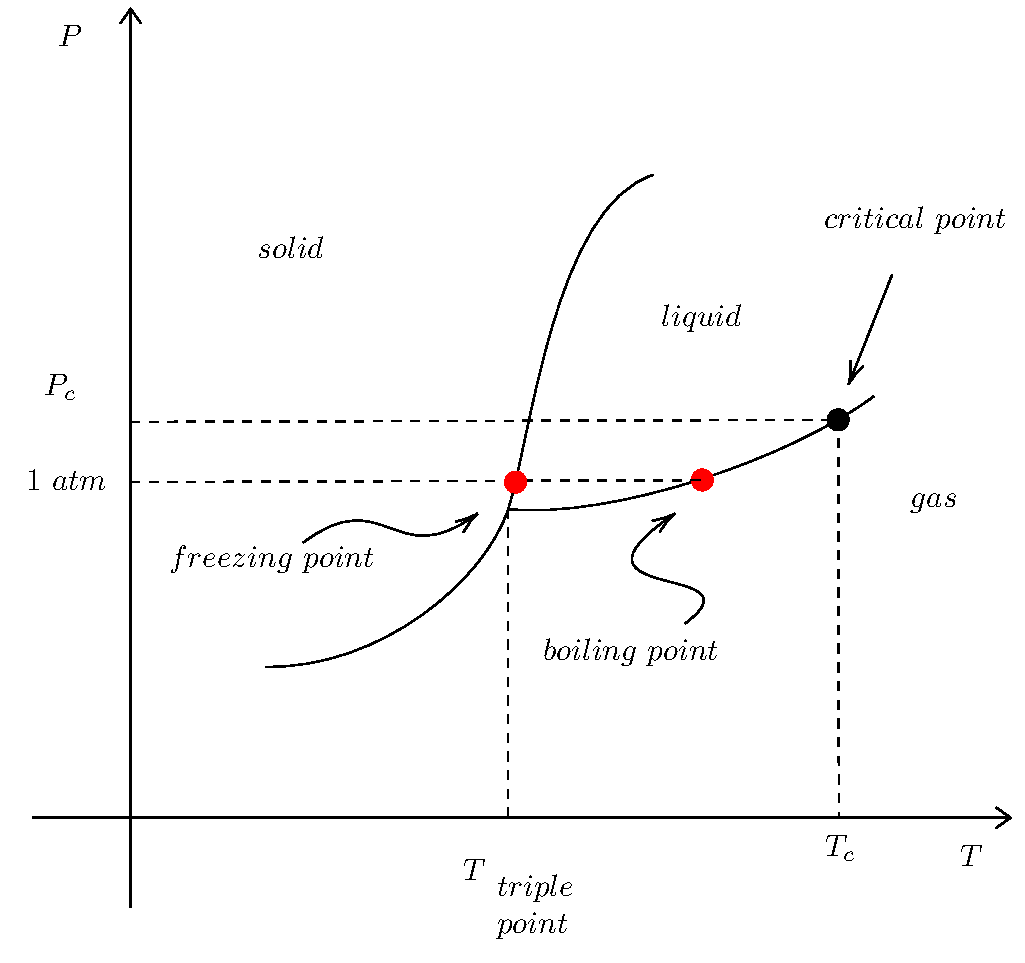
\includegraphics[width=0.8\textwidth]{../lessons/2_image/10.pdf}  \label{fig:} }
\end{minipage}
\caption{\label{fig:} Description}
\end{figure}


We can have a magnetization different from 0 even when the is no magnetic field.
Supposing \( P \leftrightarrow H, V \leftrightarrow M \), we have \( (P,T) \leftrightarrow (H,T) \). We have two equilibrium states that are connected continuosly, this is a first order transition. For instance consider Figure \ref{fig:2_7}, where at  the critical point the magnetization passes through zero.

\begin{figure}[h!]
\centering
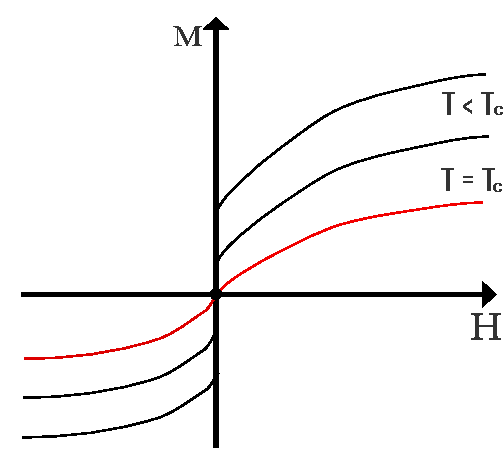
\includegraphics[width=0.5\textwidth]{../lessons/2_image/11.pdf}
\caption{\label{fig:2_7} Description.}
\end{figure}








\end{document}
